%!TEX program = xelatex
\let\stop\empty

\documentclass[12pt,a4paper]{exam-zh}

\usepackage{xeCJK}
\setCJKmainfont{Noto Serif CJK SC}
\usepackage{geometry}
\usepackage{array}
\usepackage{tikz}
\usepackage{amsmath}
\usepackage{wrapfig}
\usepackage{adjustbox}
\usepackage{enumitem}
\usepackage{fancyhdr}

\usepackage{scalerel}
\def\mcirc{\mathbin{\scalerel*{\circ}{j}}}
\def\msquare{\mathord{\scalerel*{\Box}{gX}}}
\geometry{margin=2cm}


% ----------- 调整 exam -----------


% --- 全局样式定义 ---
% 定义选择题环境：题号 1. 2.，选项 A. B. C. D. 粗体，且保留 1.5em 间距
\examsetup{
    page = {
    size = a4paper,           % 设定纸张大小 [4]
    foot-content = { - ; - }  % 页脚显示为 -1-, -2- 格式 [3]
  },
    choices = {
    label-pos = top-left,
    column-sep = 1em,
    label-pos = auto,
    label-sep = 0.5em,
    max-columns = 4
    },
  question = {
    top-sep    = 1em, % 调整题目上方的垂直距离（默认值为 .5em plus .5em minus .2em）
    bottom-sep = 1em  % 调整题目下方的垂直距离（默认值为 .5em plus .5em minus .2em）
  },
    paren = {
    show-paren = false  % 设置为 false 则不显示括号 [3, 4]
  },
    choices = {
    label = \textbf{\Alph*}
  }, 
%     solution = {
%     show-solution = show-move, % 答案自动移动到卷末
%     label-content = {参考答案},  % 答案区的标题文字
%     show-qed = true            % 在解答末尾显示结束符号 ◻ 
%   }
}

% ==========================
% 卷面变量设置（只需改这里）
% ==========================
% ==========================
% 卷面变量设置（只需改这里）
% ==========================
\newcommand{\paperlevel}{高中一}
\newcommand{\papersubject}{数学 试卷一}
\newcommand{\schoolname}{金宝培元独立中学}
\newcommand{\examname}{半年考}
\newcommand{\classinfo}{S1(Y / H)}
\newcommand{\examdate}{19-5-2026}
\newcommand{\examtime}{12:10-12:55}
\newcommand{\questiontotal}{16}
\newcommand{\paperpercentage}{40\%}
\newcommand{\setterteacher}{蔡杰庆师}
\newcommand{\reviewteacher}{王萌师}
\newcommand{\auditteacher}{雷泳健师}

\makeatletter
\newcounter{answerkeyquestion}
\let\answerkeytotal\questiontotal
\let\originalparen\paren
\newcommand{\answerkeyitems}{}
\newcommand{\addanswerkeyitem}[2]{%
  \pgfmathtruncatemacro{\row}{ifthenelse(#1<=\cols,0,1)}%
  \pgfmathtruncatemacro{\col}{mod(#1-1,\cols)}%
  \pgfmathsetlengthmacro{\x}{\col*\boxw}%
  \pgfmathsetlengthmacro{\y}{-\row*\boxh}%
  \draw (\x,\y) rectangle ++(\boxw,\boxh);%
  \node[anchor=north west] at (\x+\offset,\y+\boxh-\offset) {\textbf{#1.}};%
  \node at (\x+0.6*\boxw,\y+0.45*\boxh) {\Large\textbf{#2}};%
}
\renewcommand{\paren}[1][]{%
  \originalparen[#1]%
  \edef\answerkeytemp{#1}%
  \ifx\answerkeytemp\@empty\else
    \stepcounter{answerkeyquestion}%
    \begingroup
      \edef\x{\endgroup
        \noexpand\g@addto@macro\noexpand\answerkeyitems{\noexpand\addanswerkeyitem{\theanswerkeyquestion}{#1}}}%
    \x
  \fi
}
\makeatother

\begin{document}

% ==========================
% 三栏标题区
% ==========================
\noindent
\begin{tabular*}{\textwidth}{@{\extracolsep{\fill}} p{0.3\textwidth} p{0.35\textwidth} p{0.3\textwidth}}

\raggedright
\textbf{\paperlevel}\\[0.2em]
\textbf{}{\papersubject}\\[0.4em]
姓名：\underline{\hspace{3cm}} &

\centering
\textbf{\schoolname}\\[0.2em]
\textbf{\examname}\\[0.4em]
班级：\classinfo&

\raggedright
日期：\examdate\\[0.2em]
时间：\examtime\\[0.4em]
得分：\underline{\hspace{2.5cm}} \\

\end{tabular*}

\begin{flushleft}
考生须知： 
选出正确的答案，用蓝或黑色的原子笔将答案的相应选项字母填入本页特备作答栏。
\end{flushleft}

% =========================
% 答题栏
% =========================
\begin{flushleft}
\textbf{特备答题栏:}
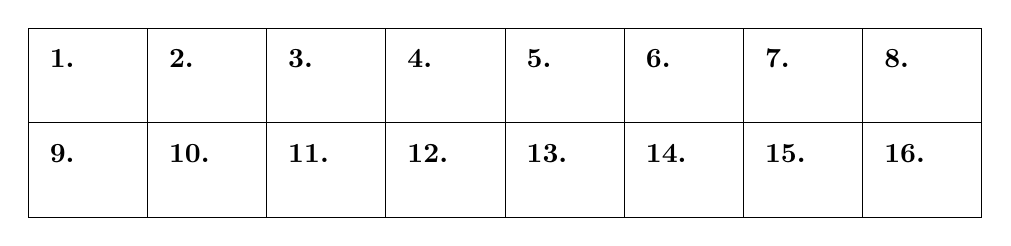
\begin{tikzpicture}
  % ---- 根据题数自动设置：16题为 8×2，20题为 10×2 ----
  \pgfmathtruncatemacro{\cols}{ifthenelse(\answerkeytotal<=16,8,10)}
  \pgfmathsetlengthmacro{\boxw}{(\linewidth-0.4pt)/\cols}
  \pgfmathsetlengthmacro{\boxh}{1.2cm}
  \pgfmathsetlengthmacro{\offset}{0.15cm}

  \foreach \num in {1,...,\answerkeytotal} {
    \pgfmathtruncatemacro{\row}{ifthenelse(\num<=\cols,0,1)}
    \pgfmathtruncatemacro{\col}{mod(\num-1,\cols)}
    \pgfmathsetlengthmacro{\x}{\col*\boxw}
    \pgfmathsetlengthmacro{\y}{-\row*\boxh}
    \draw (\x,\y) rectangle ++(\boxw,\boxh);
    \node[anchor=north west] at (\x+\offset,\y+\boxh-\offset) {\textbf{\num.}};
  }
\end{tikzpicture}

\end{flushleft}

% --- A部分：选择题 (开始) ---
\textbf{选择题：\questiontotal 题全做 \(\paperpercentage\)}

%1.
\begin{question}
    下列关于根式大小比较的选项中，正确的是： \paren[C]
    \begin{choices}
        \item $2\sqrt{3} > 3\sqrt{2}$ 
        \item $\sqrt[3]{5} < \sqrt{2}$ 
        \item $3\sqrt{5} < 4\sqrt{3}$ 
        \item $\sqrt[3]{3} > \sqrt{3}$
    \end{choices}
\end{question}

\begin{solution}
    \textbf{解析：}
    \begin{itemize}
        \item A: $2\sqrt{3} = \sqrt{12} < \sqrt{18} = 3\sqrt{2} \quad (\times)$
        \item B: $\sqrt[3]{5} = \sqrt[6]{25} > \sqrt[6]{8} = \sqrt{2} \quad (\times)$
        \item C: $3\sqrt{5} = \sqrt{45} < \sqrt{48} = 4\sqrt{3} \quad (\checkmark)$
        \item D: $\sqrt[3]{3} = \sqrt[6]{9} < \sqrt[6]{27} = \sqrt{3} \quad (\times)$
    \end{itemize}
    故选 C。
\end{solution}

%2.
\begin{question}
    若 $x > 0$，将 $\sqrt[3]{x^2} \cdot \sqrt[6]{x}$ 化简为最简根式。 \paren[B]
    \begin{choices}
        \item $\sqrt{x}$ \item $\sqrt[6]{x^5}$ \item $\sqrt[3]{x}$ \item $x$
    \end{choices}
\end{question}

\begin{solution}
    \textbf{解析：} \\
    $\sqrt[3]{x^2} \cdot \sqrt[6]{x} = x^{\frac{2}{3}} \cdot x^{\frac{1}{6}} = x^{\frac{4}{6} + \frac{1}{6}} = x^{\frac{5}{6}} = \sqrt[6]{x^5}$ \\
    故选 B。
\end{solution}

\begin{question}
    已知线段 $AB$ 的端点坐标分别为 $A(1, 2)$ 和 $B(4, 8)$，点 $P$ 在线段 $AB$ 上，且 $AP:PB = 1:2$，则点 $P$ 的坐标是： \paren[A]
    \begin{choices}
        \item $(2, 4)$ \item $(3, 6)$ \item $(2.5, 5)$ \item $(5, 10)$
    \end{choices}
\end{question}

\begin{solution}
    \textbf{解析：} \\
    根据线段的定比分点公式，若点 $A(x_1, y_1)$，$B(x_2, y_2)$，且点 $P$ 分有向线段 $AB$ 的比为 $\lambda = \frac{AP}{PB}$，则 $P$ 点坐标为： \\
    $x = \frac{x_1 + \lambda x_2}{1 + \lambda}$， $y = \frac{y_1 + \lambda y_2}{1 + \lambda}$。 \\
    本题中 $\lambda = \frac{1}{2}$，代入已知坐标： \\
    $x = \frac{1 + \frac{1}{2} \times 4}{1 + \frac{1}{2}} = \frac{3}{\frac{3}{2}} = 2$ \\
    $y = \frac{2 + \frac{1}{2} \times 8}{1 + \frac{1}{2}} = \frac{6}{\frac{3}{2}} = 4$ \\
    所以点 $P$ 的坐标为 $(2, 4)$。 \\
    故选 A。
\end{solution}

\begin{question}
    已知点 $A(1, 2)$ 和 $B(4, 5)$，点 $P$ 在线段 $AB$ 的延长线上，且 $AP:PB = 2:1$，则点 $P$ 的坐标是： \paren[C]
    \begin{choices}
        \item $(3, 4)$ \item $(-2, -1)$ \item $(7, 8)$ \item $(2, 3)$
    \end{choices}
\end{question}
\begin{solution}
    \textbf{解析：} \\
    因为点 $P$ 在线段 $AB$ 的延长线上，所以点 $P$ 为线段 $AB$ 的外分点。 \\
    由 $|AP|:|PB| = 2:1$ 且 $P$ 在 $B$ 点外侧可知，点 $P$ 分有向线段 $AB$ 的定比为负值，即 $\lambda = -2$。 \\
    根据定比分点坐标公式 $x = \frac{x_1 + \lambda x_2}{1 + \lambda}$， $y = \frac{y_1 + \lambda y_2}{1 + \lambda}$，代入已知数据可得： \\
    $x = \frac{1 + (-2) \times 4}{1 + (-2)} = \frac{1 - 8}{-1} = 7$ \\
    $y = \frac{2 + (-2) \times 5}{1 + (-2)} = \frac{2 - 10}{-1} = 8$ \\
    所以点 $P$ 的坐标为 $(7, 8)$。 \\
    \textbf{干扰项分析：} \\
    若误当作内分点（代入 $\lambda = 2$），会计算出 $(3, 4)$ 从而错选 A；若误将比例看作 $|AP|:|PB| = 1:2$ 的外分点（代入 $\lambda = -\frac{1}{2}$），会计算出 $(-2, -1)$ 从而错选 B。 \\
    故选 C。
\end{solution}

\begin{question}
    计算 $\displaystyle \sqrt{12} + \sqrt{\frac{1}{3}} - \frac{6}{\sqrt{3}} + \sqrt{27}$  。\paren[C]
    \begin{choices}
        \item $\displaystyle 2\sqrt{3}$ 
        \item $\displaystyle 3\sqrt{3}$ 
        \item $\displaystyle \frac{10\sqrt{3}}{3}$ 
        \item $\displaystyle \frac{13\sqrt{3}}{3}$
    \end{choices}
\end{question}

\newpage
\begin{question}
    求右图中三角形 $ABC$ 的面积。 \paren[C]
    
    \vspace{0cm}
    \begin{minipage}{0.4\textwidth}
        \begin{choices}
            \item 8.5 
            \item 9.0 
            \item 9.5 
            \item 10.0
        \end{choices}
    \end{minipage}%
    \begin{minipage}{0.6\textwidth}
        \centering
        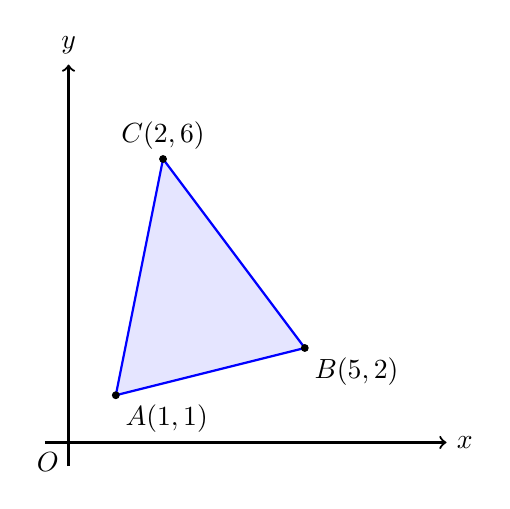
\begin{tikzpicture}[scale=0.6]
            % 画浅色网格辅助线
            % \draw[help lines, color=gray!30, dashed] (0,0) grid (6,7);
            
            % 画 x 轴和 y 轴
            \draw[->, thick] (-0.5,0) -- (8,0) node[right] {$x$};
            \draw[->, thick] (0,-0.5) -- (0,8) node[above] {$y$};
            
            % 原点
            \node[below left] at (0,0) {$O$};
            
            % 定义三角形顶点坐标
            \coordinate (A) at (1,1);
            \coordinate (B) at (5,2);
            \coordinate (C) at (2,6);
            
            % 绘制三角形并填充浅蓝色
            \draw[thick, blue, fill=blue!10] (A) -- (B) -- (C) -- cycle;
            
            % 画出顶点并标出坐标
            \filldraw[black] (A) circle (2pt) node[below right] {$A(1,1)$};
            \filldraw[black] (B) circle (2pt) node[below right] {$B(5,2)$};
            \filldraw[black] (C) circle (2pt) node[above] {$C(2,6)$};
        \end{tikzpicture}
    \end{minipage}
\end{question}


\begin{solution}
    \textbf{解析：}
    \begin{itemize}
        \item \textbf{解法1（割补法）：} 构造包围三角形的矩形（长 $4$ 宽 $5$），减去三个直角三角形。\\
        $S_{\text{矩形}} = 4 \times 5 = 20$ \\
        $S_1 = \frac{1}{2} \times 4 \times 1 = 2$ \\
        $S_2 = \frac{1}{2} \times 3 \times 4 = 6$ \\
        $S_3 = \frac{1}{2} \times 1 \times 5 = 2.5$ \\
        $S_{ABC} = 20 - 2 - 6 - 2.5 = 9.5 \quad (\checkmark)$
        
        \item \textbf{解法2（鞋带公式）：} \\
        $S_{ABC} = \frac{1}{2} |(x_A y_B + x_B y_C + x_C y_A) - (y_A x_B + y_B x_C + y_C x_A)|$ \\
        $S_{ABC} = \frac{1}{2} |(1 \times 2 + 5 \times 6 + 2 \times 1) - (1 \times 5 + 2 \times 2 + 6 \times 1)|$ \\
        $S_{ABC} = \frac{1}{2} |(2 + 30 + 2) - (5 + 4 + 6)|$ \\
        $S_{ABC} = \frac{1}{2} |34 - 15| = 9.5 \quad (\checkmark)$
    \end{itemize}
    故选 C。
\end{solution}

\begin{question}
    已知平面直角坐标系中点 $A(1, 4)$，点 $B$ 落在 $x$ 轴上。若点 $A$ 与点 $B$ 之间的距离为 $5$，则点 $B$ 的坐标为： \paren[D]
    \begin{choices}
        \item $(4, 0)$ \item $(-2, 0)$ \item $(3, 0)$ 或 $(-3, 0)$ \item $(4, 0)$ 或 $(-2, 0)$
    \end{choices}
\end{question}

\begin{solution}
    \textbf{解析：} \\
    1. 因为点 $B$ 在 $x$ 轴上，可设点 $B$ 的坐标为 $(x, 0)$。 \\
    2. 根据两点间距离公式 $|AB| = \sqrt{(x - 1)^2 + (0 - 4)^2} = 5$。 \\
    3. 两边平方得：$(x - 1)^2 + (-4)^2 = 25$。 \\
    4. 整理得：$(x - 1)^2 + 16 = 25 \Rightarrow (x - 1)^2 = 9$。 \\
    5. 开方得：$x - 1 = 3$ 或 $x - 1 = -3$。 \\
    6. 解得：$x = 4$ 或 $x = -2$。 \\
    所以点 $B$ 的坐标为 $(4, 0)$ 或 $(-2, 0)$。 \\
    故选 D。
\end{solution}



\begin{solution}
    \textbf{解析：} \\
    {\Large
    \begin{itemize}
        \item $\displaystyle \sqrt{12} = 2\sqrt{3}$
        \item $\displaystyle \sqrt{\frac{1}{3}} = \frac{\sqrt{3}}{3}$
        \item $\displaystyle \frac{6}{\sqrt{3}} = \frac{6\sqrt{3}}{3} = 2\sqrt{3}$
        \item $\displaystyle \sqrt{27} = 3\sqrt{3}$
    \end{itemize}
    }
    \textbf{合并同类根式：} \\
    $\displaystyle 2\sqrt{3} + \frac{\sqrt{3}}{3} - 2\sqrt{3} + 3\sqrt{3}$ \\
    $\displaystyle = (2 - 2 + 3)\sqrt{3} + \frac{\sqrt{3}}{3}$ \\
    $\displaystyle = 3\sqrt{3} + \frac{\sqrt{3}}{3}$ \\
    $\displaystyle = \frac{10\sqrt{3}}{3}$ \\
    故选 C。
\end{solution}

\begin{question}
    化简二次不尽根式 $\displaystyle \sqrt{7 - 4\sqrt{3}}$。 \paren[B]
    \begin{choices}
        \item $\displaystyle \sqrt{3} - 2$ 
        \item $\displaystyle 2 - \sqrt{3}$ 
        \item $\displaystyle \sqrt{3} - \sqrt{2}$ 
        \item $\displaystyle 2 + \sqrt{3}$
    \end{choices}
\end{question}

\begin{solution}
    \textbf{解析：} \\
    我们要将 $\displaystyle \sqrt{7 - 4\sqrt{3}}$ 化简，目标是将其被开方数凑成一个完全平方式。 \\
    
    1. **观察与变形**：将 $4\sqrt{3}$ 写成 $2\sqrt{ab}$ 的形式：
    $\displaystyle 4\sqrt{3} = 2 \times 2\sqrt{3} = 2\sqrt{4 \times 3} = 2\sqrt{12}$。 \\
    
    2. **寻找数值**：我们需要找到两个数 $x$ 和 $y$，使得：
    $\begin{cases} x + y = 7 \\ xy = 12 \end{cases}$ \\
    通过观察或解方程可知，$x=4$，$y=3$ 满足条件。 \\
    
    3. **构造完全平方**：
    $\displaystyle 7 - 4\sqrt{3} = 4 + 3 - 2\sqrt{4 \times 3} = (\sqrt{4})^2 + (\sqrt{3})^2 - 2\sqrt{4}\sqrt{3} = (2 - \sqrt{3})^2$。 \\
    
    4. **开方得出结果**：
    $\displaystyle \sqrt{7 - 4\sqrt{3}} = \sqrt{(2 - \sqrt{3})^2} = |2 - \sqrt{3}|$。 \\
    由于 $2 = \sqrt{4} > \sqrt{3}$，所以 $2 - \sqrt{3}$ 为正数。 \\
    结果为 $\displaystyle 2 - \sqrt{3}$。 \\
    
    \textbf{易错点}：选项 A 的数值虽然正确，但根式化简结果必须为非负数，$\sqrt{3}-2$ 是负数，故排除。 \\
    故选 B。
\end{solution}

\begin{question}
    已知 $x > 0$ 且 $x \neq 1$，化简 $\displaystyle \frac{x-1}{\sqrt{x}+1} \cdot \sqrt{x}$ 。 \paren[B]
    \begin{choices}
        \item $\displaystyle x + \sqrt{x}$ 
        \item $\displaystyle x - \sqrt{x}$ 
        \item $\displaystyle \sqrt{x} - 1$ 
        \item $\displaystyle x - 1$
    \end{choices}
\end{question}

\begin{solution}
    \textbf{解析：} \\
    这道题有两种常用的处理方法：
    
    \textbf{方法一：分母有理化} \\
    将第一项的分式分子、分母同时乘以 $(\sqrt{x}-1)$：
    $$\frac{(x-1)(\sqrt{x}-1)}{(\sqrt{x}+1)(\sqrt{x}-1)} \cdot \sqrt{x}$$
    根据平方差公式 $(a+b)(a-b)=a^2-b^2$，分母变为 $(\sqrt{x})^2 - 1^2 = x-1$：
    $$\frac{(x-1)(\sqrt{x}-1)}{x-1} \cdot \sqrt{x}$$
    约去 $(x-1)$，得：
    $$(\sqrt{x}-1) \cdot \sqrt{x} = (\sqrt{x})^2 - \sqrt{x} = x - \sqrt{x}$$

    \textbf{方法二：分子因式分解（更简便）} \\
    观察到分子 $x-1$ 可以写成 $(\sqrt{x})^2 - 1^2$，利用平方差公式展开：
    $$\frac{(\sqrt{x}+1)(\sqrt{x}-1)}{\sqrt{x}+1} \cdot \sqrt{x}$$
    直接约去 $(\sqrt{x}+1)$，得：
    $$(\sqrt{x}-1) \cdot \sqrt{x} = x - \sqrt{x}$$
    
    故选 B。
\end{solution}

\begin{question}
    已知直线 $ax + by = 2$ 的斜率为 $-\dfrac{1}{2}$，且该直线经过点 $(-4, 1)$，则 $a$ 的值为： \paren[C]
    \begin{choices}
        \item $-2$ \item $-1$ \item $1$ \item $2$
    \end{choices}
\end{question}

\begin{solution}
    \textbf{解析} $\blacktriangleright$ \\
    本题可以通过直线的斜率性质和点在直线上的代数关系来求解。

    1. **利用斜率求 $a$ 与 $b$ 的关系**：
    将直线的一般式 $ax + by = 2$ 化为斜截式：
    $by = -ax + 2 \implies y = -\dfrac{a}{b}x + \dfrac{2}{b}$（假设 $b \neq 0$）。
    根据题意，斜率 $k = -\dfrac{a}{b} = -\dfrac{1}{2}$。
    由此可得：$\dfrac{a}{b} = \dfrac{1}{2} \implies b = 2a$。 \hfill ①

    2. **利用点在直线上求解**：
    因为直线经过点 $(-4, 1)$，将坐标代入原方程 $ax + by = 2$：
    $a(-4) + b(1) = 2 \implies -4a + b = 2$。 \hfill ②

    3. **联立方程组**：
    将 ① 式 $b = 2a$ 代入 ② 式中：
    $-4a + 2a = 2$
    $-2a = 2$
    解得：$a = -1$。

    \textbf{注意}：虽然题目只要求 $a$，我们可以算出 $b = 2a = -2$。此时方程为 $-x - 2y = 2$，验证斜率确实为 $-\dfrac{1}{2}$ 且通过点 $(-4, 1)$。

    故选 B。
\end{solution}

\begin{question}
    已知直线 $mx + (n-1)y = 4$ 与直线 $(m-2)x + 3ny = 5$ 相交于点 $(2, -1)$，则 $m$ 与 $n$ 的值分别为： \paren[C]
    \begin{choices}
        \item $m = -3, n = 0$ \item $m = -1, n = -5$ \item $m = 0, n = -3$ \item $m = 3, n = 3$
    \end{choices}
\end{question}

\begin{solution}
    \textbf{解析：} \\
    因为两条直线相交于点 $(2, -1)$，所以该点的坐标同时满足这两条直线的解析式。 \\
    将 $x = 2, y = -1$ 分别代入两条直线的方程中，可得关于 $m, n$ 的二元一次方程组：
    $$
    \begin{cases}
    m(2) + (n-1)(-1) = 4 \\
    (m-2)(2) + 3n(-1) = 5
    \end{cases}
    $$
    去括号并移项化简该方程组，得：
    $$
    \begin{cases}
    2m - n + 1 = 4 \\
    2m - 4 - 3n = 5
    \end{cases}
    \implies
    \begin{cases}
    2m - n = 3 \quad \text{①} \\
    2m - 3n = 9 \quad \text{②}
    \end{cases}
    $$
    利用加减消元法求解，用 ① 式减去 ② 式，消去 $m$，得：
    $$(2m - n) - (2m - 3n) = 3 - 9$$
    $$2n = -6 \implies n = -3$$
    将 $n = -3$ 代入 ① 式，得：
    $$2m - (-3) = 3 \implies 2m + 3 = 3 \implies 2m = 0 \implies m = 0$$
    所以解得 $m = 0, n = -3$。选项已按照 $m$ 的值从小到大进行了排列。 \\
    故选 C。
\end{solution}

\newpage
\begin{question}
    已知直线的方程为 $ax + by + c = 0$，若满足 $ab > 0$ 且 $bc < 0$，则该直线的图像可能是： \paren[B]
    
    \vspace{0.5cm}
    \begin{choices}
    \item
    \begin{minipage}{0.22\textwidth}
        \centering
        \begin{tikzpicture}[scale=0.6]
            \draw[->] (-2,0) -- (2,0) node[right] {\tiny $x$};
            \draw[->] (0,-2) -- (0,2) node[above] {\tiny $y$};
            \draw[thick, blue] (-1.5,-1.5) -- (1.5,1.5);
        \end{tikzpicture}
    \end{minipage}
    \item 
    \begin{minipage}{0.22\textwidth}
        \centering
        \begin{tikzpicture}[scale=0.6]
            \draw[->] (-2,0) -- (2,0) node[right] {\tiny $x$};
            \draw[->] (0,-2) -- (0,2) node[above] {\tiny $y$};
            \draw[thick, blue] (-1.5,1.5) -- (1.5,-0.5);
        \end{tikzpicture}
    \end{minipage}
    \item
    \begin{minipage}{0.22\textwidth}
        \centering
        \begin{tikzpicture}[scale=0.6]
            \draw[->] (-2,0) -- (2,0) node[right] {\tiny $x$};
            \draw[->] (0,-2) -- (0,2) node[above] {\tiny $y$};
            \draw[thick, blue] (-1.5,0.5) -- (1.5,-1.5);
        \end{tikzpicture}
    \end{minipage}
    \item
    \begin{minipage}{0.22\textwidth}
        \centering
        \begin{tikzpicture}[scale=0.6]
            \draw[->] (-2,0) -- (2,0) node[right] {\tiny $x$};
            \draw[->] (0,-2) -- (0,2) node[above] {\tiny $y$};
            \draw[thick, blue] (-1.5,-0.5) -- (1.5,1.5);
        \end{tikzpicture}
    \end{minipage}
\end{choices}
\end{question}

\begin{solution}
    \textbf{解析：} \\
    1. 将一般式方程 $ax + by + c = 0$ 转化为斜截式：$y = -\frac{a}{b}x - \frac{c}{b}$。
    \begin{itemize}
        \item 斜率 $k = -\frac{a}{b}$
        \item $y$ 轴截距 $n = -\frac{c}{b}$
    \end{itemize}
    
    2. **判断符号**：
    \begin{itemize}
        \item 因为 $ab > 0$，说明 $a, b$ 同号，则 $\frac{a}{b} > 0$，故斜率 $k = -\frac{a}{b} < 0$。直线应向右下方倾斜（排除 A, D）。
        \item 因为 $bc < 0$，说明 $b, c$ 异号，则 $\frac{c}{b} < 0$，故截距 $n = -\frac{c}{b} > 0$。直线与 $y$ 轴的交点应在原点上方。
    \end{itemize}
    
    3. **结论**：
    斜率为负且 $y$ 轴截距为正的图像只有 B。
    
    故选 B。
\end{solution}

\begin{question}
    在平面直角坐标系中，点 $P(2, -1)$ 到直线 $l: 4x + 3y + 5 = 0$ 的距离为： \paren[D]
    \begin{choices}
        \item $1$ \item $1.5$ \item $1.8$ \item $2$
    \end{choices}
\end{question}

\begin{solution}
    \textbf{解析：} \\
    已知点 $P(x_0, y_0) = (2, -1)$，直线方程为 $4x + 3y + 5 = 0$，其中系数 $A=4, B=3, C=5$。 \\
    利用点到直线的距离公式：
    $$\displaystyle d = \frac{|Ax_0 + By_0 + C|}{\sqrt{A^2 + B^2}}$$
    代入数据计算：
    $$\displaystyle d = \frac{|4 \times 2 + 3 \times (-1) + 5|}{\sqrt{4^2 + 3^2}}$$
    $$\displaystyle d = \frac{|8 - 3 + 5|}{\sqrt{16 + 9}}$$
    $$\displaystyle d = \frac{|10|}{\sqrt{25}} = \frac{10}{5} = 2$$
    计算结果为 $2$，选项已按从小到大排列。 \\
    故选 D。
\end{solution}




\begin{question}
    已知实数 $x, y$ 满足 $y < x < 0$，则下列不等式中一定正确的是： \paren[B]
    \begin{choices}
        \item $x^2 > y^2$ 
        \item $\displaystyle \frac{1}{x} < \frac{1}{y}$ 
        \item $x + y > 0$ 
        \item $xy < 0$
    \end{choices}
\end{question}

\begin{solution}
    \textbf{解析：} \\
    已知 $y < x < 0$，说明 $x, y$ 均为负数，且 $y$ 在数轴上位于 $x$ 的左侧（即 $|y| > |x|$）。我们可以结合不等式性质推导，也可以使用\textbf{特殊值法}（例如令 $x = -1, y = -2$）来快速验证。

    \begin{itemize}
        \item \textbf{A 选项}：因为 $y < x < 0$，说明 $y$ 的绝对值大于 $x$ 的绝对值，平方后应有 $y^2 > x^2$。\\
        （特殊值验证：$(-1)^2 \ngtr (-2)^2$，即 $1 \ngtr 4$，故 A 错误）
        
        \item \textbf{B 选项}：根据不等式性质，当 $y < x$ 时，在不等式两边同时除以同一个正数 $xy$（因为 $x,y$ 同号，所以 $xy > 0$），不等号方向不变，即 $\frac{y}{xy} < \frac{x}{xy}$，化简得 $\frac{1}{x} < \frac{1}{y}$。\\
        （特殊值验证：$\frac{1}{-1} < \frac{1}{-2}$，即 $-1 < -0.5$，成立，故 B 正确）
        
        \item \textbf{C 选项}：因为 $x < 0$ 且 $y < 0$，两个负数相加必定为负数，即 $x + y < 0$。\\
        （特殊值验证：$-1 + (-2) = -3 \ngtr 0$，故 C 错误）
        
        \item \textbf{D 选项}：因为 $x < 0$ 且 $y < 0$，同号两数相乘得正，即 $xy > 0$。\\
        （特殊值验证：$(-1) \times (-2) = 2 \nless 0$，故 D 错误）
    \end{itemize}
    
    故选 B。
\end{solution}

\begin{question}
    不等式 $\displaystyle \left(x - \frac{3}{4}\right)\left(x - \frac{5}{7}\right) < 0$ 的解集是： \paren[A]
    \begin{choices}
        \item $\displaystyle \frac{5}{7} < x < \frac{3}{4}$ 
        \item $\displaystyle \frac{3}{4} < x < \frac{5}{7}$ 
        \item $\displaystyle x < \frac{5}{7}$ 或 $\displaystyle x > \frac{3}{4}$ 
        \item $\displaystyle x < \frac{3}{4}$ 或 $\displaystyle x > \frac{5}{7}$
    \end{choices}
\end{question}

\begin{solution}
    \textbf{解析：} \\
    本题考查一元二次不等式的解法以及分数大小的比较。
    
    1. **求根**：令 $\displaystyle \left(x - \frac{3}{4}\right)\left(x - \frac{5}{7}\right) = 0$，解得两个根分别为 $\displaystyle x_1 = \frac{3}{4}$，$\displaystyle x_2 = \frac{5}{7}$。
    
    2. **比较大小**：要想写出正确的区间，必须先判断这两个根谁大谁小。
    \begin{itemize}
        \item 找通分分母：$4$ 和 $7$ 的最小公倍数是 $28$。
        \item 转化为同分母分数：$\displaystyle \frac{3}{4} = \frac{21}{28}$，$\displaystyle \frac{5}{7} = \frac{20}{28}$。
        \item 因为 $21 > 20$，所以 $\displaystyle \frac{3}{4} > \frac{5}{7}$。
    \end{itemize}
    
    3. **确定区间**：原不等式符号为“$<$”（小于零），根据“小于取中间”的原则，解集应介于较小的根与较大的根之间。
    因此，解集为 $\displaystyle \frac{5}{7} < x < \frac{3}{4}$。
    
    \textbf{易错点提示}：
    1. **顺序陷阱**：很多学生会直接按题干中数字出现的顺序写成 $\displaystyle \frac{3}{4} < x < \frac{5}{7}$（错选 B），但这是一个空集，因为左边实际上大于右边。
    2. **口诀记混**：误用了“大于取两边”的规则（错选 C）。 \\
    故选 A。
\end{solution}

\begin{question}
    已知一元二次不等式 $x^2 - 4x + 3 < 0$，则下列哪个 $x$ 的值满足该不等式？ \paren[B]
    \begin{choices}
        \item $0$ \item $2$ \item $3$ \item $4$
    \end{choices}
\end{question}

\begin{solution}
    \textbf{解析：} \\
    解答这道选择题有两种常用的方法：
    
    \textbf{方法一：直接代入验证法（特值法）} \\
    将四个选项的值分别代入不等式的左边进行计算：
    \begin{itemize}
        \item 当 $x = 0$ 时，左边 $= 0^2 - 4 \times 0 + 3 = 3$，因为 $3 \nless 0$，所以 A 选项不满足。
        \item 当 $x = 2$ 时，左边 $= 2^2 - 4 \times 2 + 3 = 4 - 8 + 3 = -1$，因为 $-1 < 0$，所以 B 选项满足。
        \item 当 $x = 3$ 时，左边 $= 3^2 - 4 \times 3 + 3 = 9 - 12 + 3 = 0$，因为 $0 \nless 0$（原式没有等于号），所以 C 选项不满足。
        \item 当 $x = 4$ 时，左边 $= 4^2 - 4 \times 4 + 3 = 16 - 16 + 3 = 3$，因为 $3 \nless 0$，所以 D 选项不满足。
    \end{itemize}
    
    \textbf{方法二：正向求解不等式法} \\
    1. **因式分解**：将原不等式 $x^2 - 4x + 3 < 0$ 的左边利用十字相乘法进行分解，得到 $(x - 1)(x - 3) < 0$。 \\
    2. **求出解集**：对应方程的两个根为 $x_1 = 1, x_2 = 3$。根据二次项系数为正且符号为“$<$”，利用“小于取中间”的口诀，得出不等式的解集为 $1 < x < 3$。 \\
    3. **判断选项**：观察四个选项，只有选项 B 中的 $2$ 落在区间 $(1, 3)$ 内。
    
    \textbf{易错点}：学生可能会错选 C，因为他们可能在求解 $(x-1)(x-3)<0$ 时，误以为端点值也是解，忽略了不等式是严格的小于号（没有等于）。 \\
    故选 B。
\end{solution}
\newpage

\begin{center}
\textbf{参考答案}

\begin{tikzpicture}
  \pgfmathtruncatemacro{\cols}{ifthenelse(\answerkeytotal<=16,8,10)}
  \pgfmathsetlengthmacro{\boxw}{(\linewidth-0.4pt)/\cols}
  \pgfmathsetlengthmacro{\boxh}{1.2cm}
  \pgfmathsetlengthmacro{\offset}{0.15cm}

  \answerkeyitems
\end{tikzpicture}
\end{center}

\vfill % 与上方内容保持距离

\noindent
\newlength{\sigwidth}
\settowidth{\sigwidth}{（\hspace{4em}师）}

\begin{tabular*}{\textwidth}{@{\extracolsep{\fill}} l l l}
    出题： & 审题： & 审核： \\[4em]
    \rule{\sigwidth}{0.5pt} &
    \rule{\sigwidth}{0.5pt} &
    \rule{\sigwidth}{0.5pt} \\
    （\hspace{0em} \setterteacher ） &
    （\hspace{0em} \reviewteacher ） &
    （\hspace{0em} \auditteacher ） \\
\end{tabular*}


\end{document}